\documentclass{article}

\usepackage{graphicx}
\usepackage{tikz}
\usepackage{tikzsymbols}
\usetikzlibrary{calc,patterns,shapes.geometric}
\pagestyle{empty}
\usepackage[margin=0pt]{geometry}
\geometry{papersize={14in,12in}}

\def\centerarc[#1](#2)(#3:#4:#5){\draw[#1] ($(#2)+({#5*cos(#3)},{#5*sin(#3)})$) arc (#3:#4:#5);}

\begin{document}
	\begin{figure}
		\centering
		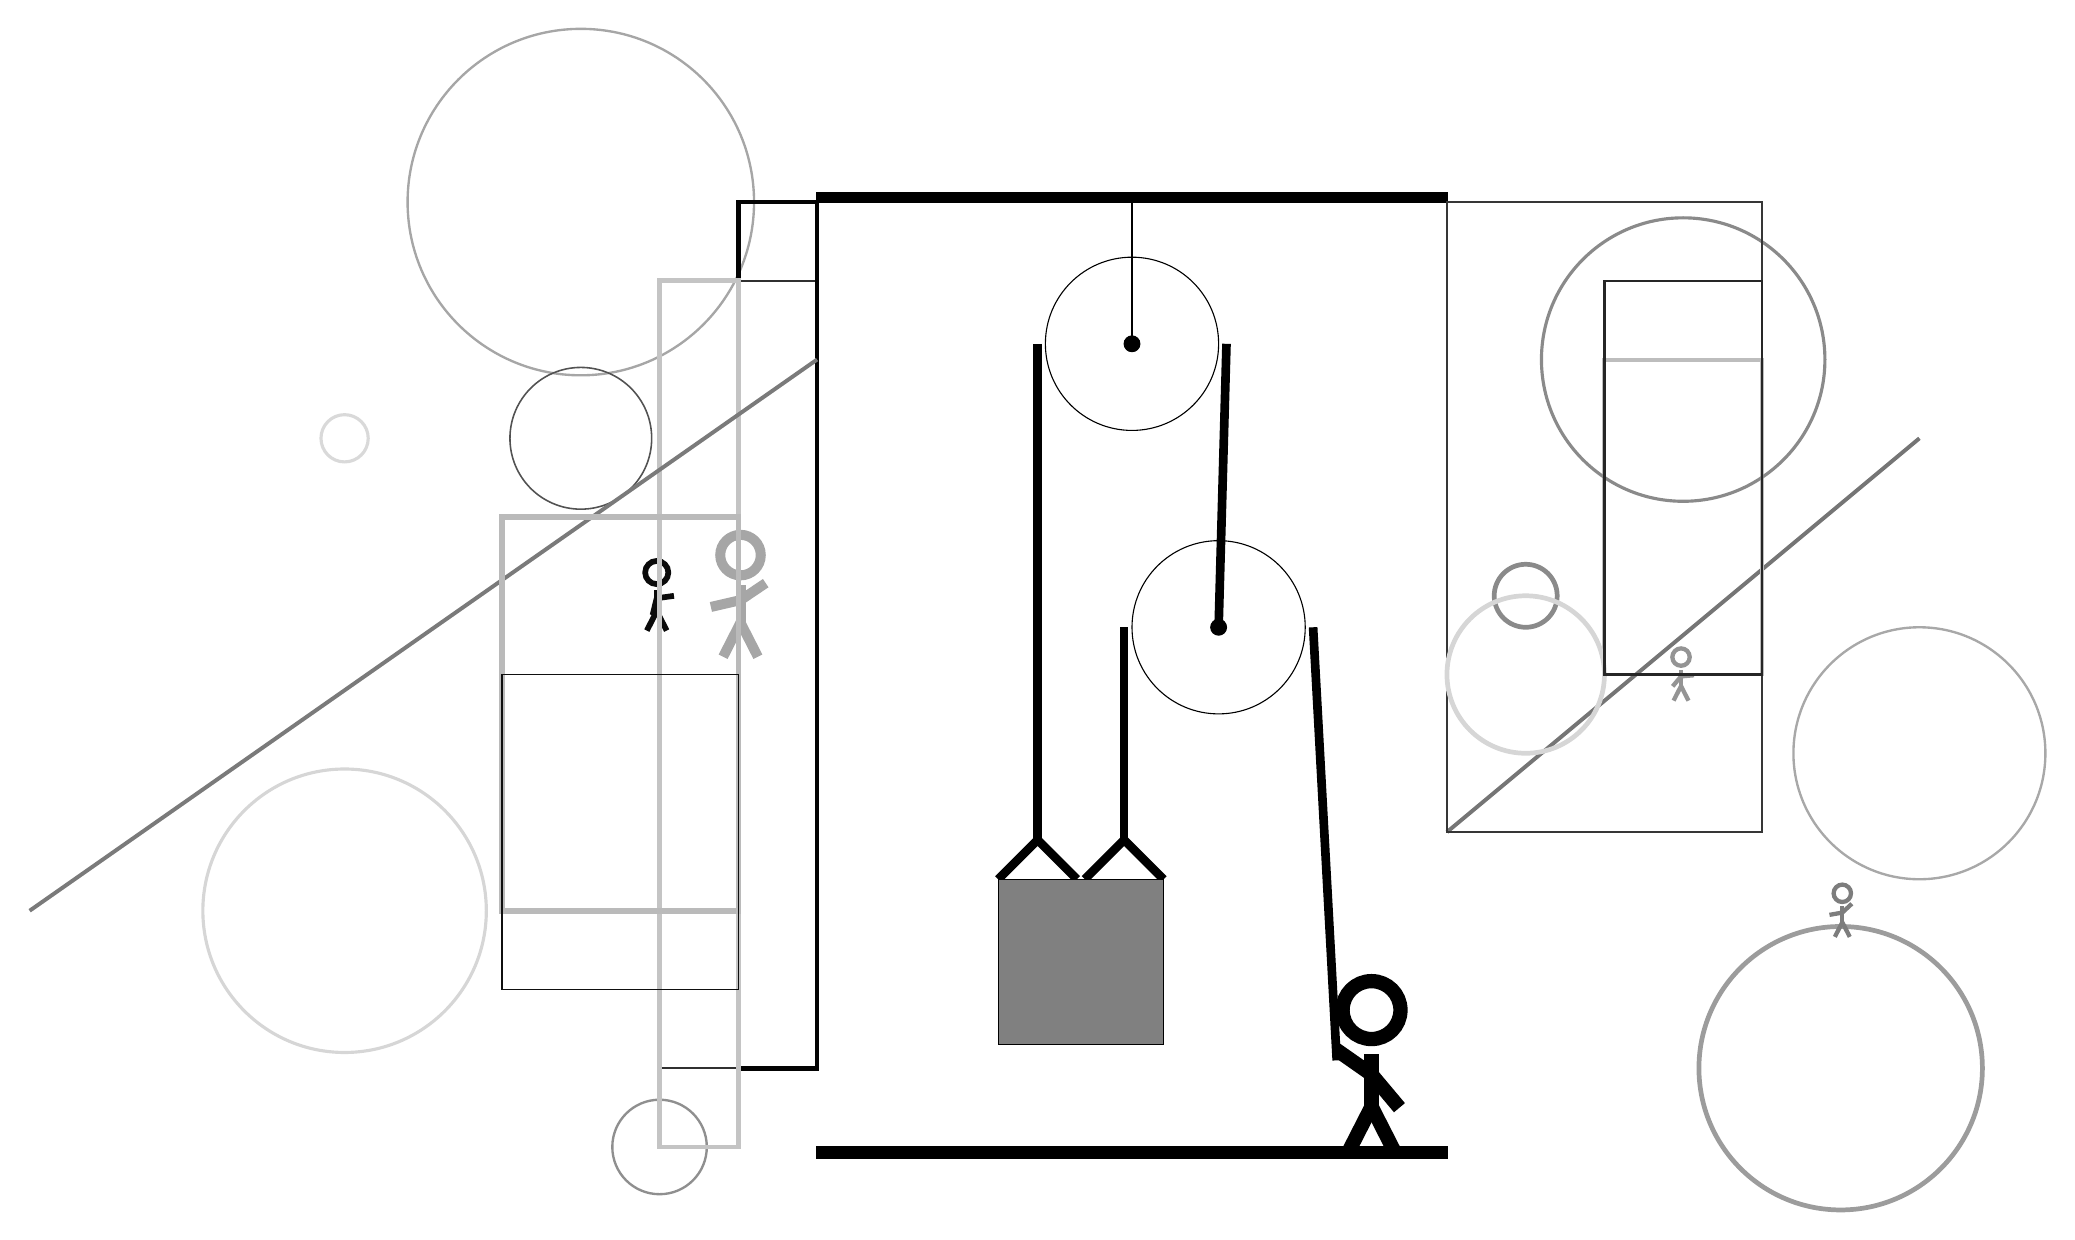
\begin{tikzpicture}
			%%%%% START %%%%%
			
			\draw[fill=black] (-2, 9) rectangle (6, 9.125);
			
			\draw (2, 7.2) circle (1.1);
			\draw[fill=black] (2, 7.2) circle (0.1);
			\draw[thick] (2, 7.2) -- (2, 9);
			
			\draw (3.1, 3.6) circle (1.1);
			\draw[fill=black] (3.1, 3.6) circle (0.1);
			
			\draw[line width = 1.1mm]  (0.3, 0.4) -- (0.8, 0.9) -- (1.3, 0.4);
			\draw[line width = 1.1mm]  (1.4, 0.4) -- (1.9, 0.9) -- (2.4, 0.4);
			\draw[fill=black!50] (0.3, 0.4) rectangle (2.4, -1.7);
			
			\draw[line width=0.5mm, color=black!54](6, 1) -- (12, 6);
			
			\node[line width=0.5mm, color=black!96] at (-4, 4) {\Strichmaxerl[4][76][8]};
			\draw[line width=0.3mm, color=black!81] (-2, 8) rectangle (-4, -2);
			\draw [line width=0.3mm, color=black!35](-5, 9) circle (2.2);
			\draw [line width=0.3mm, color=black!44](-4, -3) circle (0.6);
			\draw [line width=0.4mm, color=black!16](-8, 0) circle (1.8);
			
			\draw[line width=0.6mm, color=black!99] (-2, -2) rectangle (-3, 9);
			\draw [line width=0.4mm, color=black!15](-8, 6) circle (0.3);
			\draw[line width=0.3mm, color=black!55] (-4, -3) rectangle (-4, 7);
			\draw[line width=0.5mm, color=black!26] (8, 7) rectangle (10, 3);
			\draw [line width=0.4mm, color=black!46](9, 7) circle (1.8);
			\draw [line width=0.3mm, color=black!34](12, 2) circle (1.6);
			\draw [line width=0.6mm, color=black!39](11, -2) circle (1.8);
			
			\draw[line width=0.3mm, color=black!79] (6, 1) rectangle (10, 9);
			\draw [line width=0.6mm, color=black!46](7, 4) circle (0.4);
			\draw [line width=0.2mm, color=black!68](-5, 6) circle (0.9);
			
			\draw[line width=0.4mm, color=black!23] (-4, 8) rectangle (-4, 3);
			\draw [line width=0.6mm, color=black!16](7, 3) circle (1.0);
			\draw[line width=0.6mm, color=black!23] (-3, -3) rectangle (-4, 8);
			
			\node[line width=0.7mm, color=black!42] at (9, 3) {\Strichmaxerl[3][50][5]};
			\node[line width=0.2mm, color=black!35] at (-3, 4) {\Strichmaxerl[7][13][34]};
			\node[line width=0.3mm, color=black!51] at (11, 0) {\Strichmaxerl[3][10][43]};
			
			\draw[line width=0.5mm, color=black!52](-2, 7) -- (-12, 0);
			\draw[line width=0.3mm, color=black!85] (8, 3) rectangle (10, 8);
			\draw[line width=0.7mm, color=black!27] (-3, 5) rectangle (-6, 0);
			\draw[line width=0.2mm, color=black!94] (-3, -1) rectangle (-6, 3);
			
			\draw[line width = 1.1mm] (0.8, 7.2) -- (0.8, 0.9);
			\centerarc[line width = 1.1mm](2, 7.2)(0:180:1.2000000000000002);
			\draw[line width = 1.1mm] (3.2, 7.2) -- (3.1, 3.6);
			\draw[line width = 1.1mm] (1.9, 3.6) -- (1.9, 0.9);
			\centerarc[line width = 1.1mm](3.1, 3.6)(0:180:1.2000000000000002);
			\draw[line width = 1.1mm] (4.3, 3.6) -- (4.6, -1.9);
			
			\node at (5, -2) {\Strichmaxerl[10][-35][-50]};
			
			\draw[fill=black] (-2, -3) rectangle (6, -3.15);
			
			%%%%% END %%%%%
		\end{tikzpicture}
	\end{figure}	
\end{document}